% id: 0644
% book: RPM 중학 3-2 · 07 상자그림과 산점도
% section: 유형 08 산점도와 상관관계
% figure: crop:fig-0644-2.png
% answer: ④
% answer_source: 답지
% variant_level: 0 (원본 전사)
% 이 파일은 build.mjs 가 items.json 에서 만든다. 고칠 때는 items.json 을 고친다.
\smash{\raisebox{1.5mm}{\dmkichul{RPM 중학 3-2 0644번 · 110쪽}}}
\noindent\begin{minipage}[t]{0.58\linewidth}\vspace{0pt}\raggedright 다음 \textbf{보기} 중 두 변량 사이의 산점도가 대체로 오른쪽 그림과 같이 나타나는 것을 모두 고른 것은?\end{minipage}\hfill\begin{minipage}[t]{0.4\linewidth}\vspace{0pt}\centering \setlength{\dmfigw}{75.3pt}\ifdim\dmfigw>\linewidth\setlength{\dmfigw}{\linewidth}\fi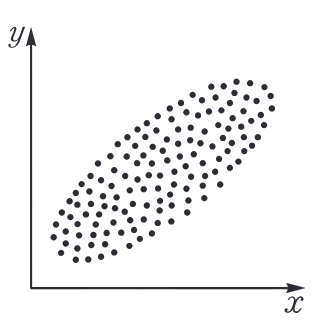
\includegraphics[width=\dmfigw]{figures/fig-0644-2.png}\end{minipage}\par
\noindent \bogi{ㄱ. 사용한 전력량과 전기 요금\\ ㄴ. 어떤 물건의 가격과 판매량\\ ㄷ. 지능 지수와 몸무게\\ ㄹ. 통학 거리와 통학 시간\\ ㅁ. 자동차의 속력과 정지할 때의 움직인 거리}
\begin{choices32}{ㄱ, ㄴ}{ㄱ, ㄷ}{ㄴ, ㄷ}{ㄱ, ㄹ, ㅁ}{ㄷ, ㄹ, ㅁ}\end{choices32}
